% !TEX root = main.tex
\section{The experiment}
In this section we now describe the experiments we conducted.
We first present the general set-up of the experiments, then we will describe how we defined the base cases for each experiment in order to perform tests against them.
After that, we will go through the deception techniques we used to deceive the users in order to avoid bias in the results, and finally we will describe in details the specific experiments.
As a further note we'll go briefly into the data collection and analysis process.

\subsection{Testers}
The testers were graduate and undergraduate students found in a public library, whose participation was completely voluntary.

\subsection{Set up}
The testers interacted with an iPad application in which they are told to perform actions on a balloon on the screen. The iPad choice has been determined by the will of keeping the interaction as natural as possible in order not to make it influent over the measurement of the synchronization aspects of the experiments; the touch interaction on an iPad screen seemed to be the most suitable choice.
The testers were wearing headphones while interacting with the iPad applications and the approximate duration of the tests per each user was about 2 minutes.

\subsection{Deception}
Due to the configuration discussed above, there could have been the risk that a tester would have understood the purpose of the test. In fact she could have got the purpose of the test noticing that we were enforcing her to wear headphones. This could have brought some bias in the data collection as the tester could have voluntarily tried to synchronize with the soundtrack.
We then try to deceive her by explaining the presence of the headphones as way to increase the concentration on the task, avoiding outside interference.

Moreover the task itself was presented as a beta testing activity for a video-game design course, so the testers thought of being testing an in-development game, rather than participating to an experiment.

\subsection{Base cases}
\label{sec:base-cases}
We are clearly interested to the effects the background tempo produces on the participants, therefore both of the experiments run with a background beat.
Since we wanted to see whether there is a synchronization between the background tempo and the actions the user is performing, we first of all set a base case for all the experiments.
By base case here we mean a test run of the experiments \emph{without} music across multiple users, in order to determine an average measure for each experiment (we will discuss about the measures later in Section~\ref{sec:measures}).

\subsection{The tempo}
We wanted a background soundtrack as regular as possible in order to increase the precision of the measure, but we wanted also to avoid plain beat sequences, that could result annoying for the testers.

Our final choice was the famous Tetris\textsuperscript{\texttrademark} soundtrack, taken in its original version from the Nintendo\textsuperscript{\texttrademark} GameBoy\textsuperscript{\texttrademark} game, having a very regular and clear beat although being pleasant to the testers.

We then changed the BPM (beats per minute) of the song according to the different experiments.

For the first experiment (\nameref{sec:test1}) we set the BPM to 130, which is slightly faster than the base case (see Section~\ref{sec:base-cases}).

For the second one we instead tried to slow down the tapping rate by setting the BPM to 153, whereas the base case was \todo[inline]{Insert data of basecases}.

\subsection{\testfirst}
\label{sec:test1}
The first test consisted of an application where the user was asked to tap a red balloon present on the screen. In Figure~\ref{fig:test1} is shown an in-game screen shot of the application.

Every time the user tapped on the balloon, this instantaneously moved to a different random location on the screen. The result of such an interaction is the user chasing the balloon around the screen, repeatedly tapping on it. This went on for 45 seconds.
The whole sequence is sent in real time to a web-server we developed and stored on a remote database for further analysis.

\begin{figure}[h!t]
\label{fig:test1}
\centering
	{\setlength{\fboxsep}{0pt}
	 \fbox{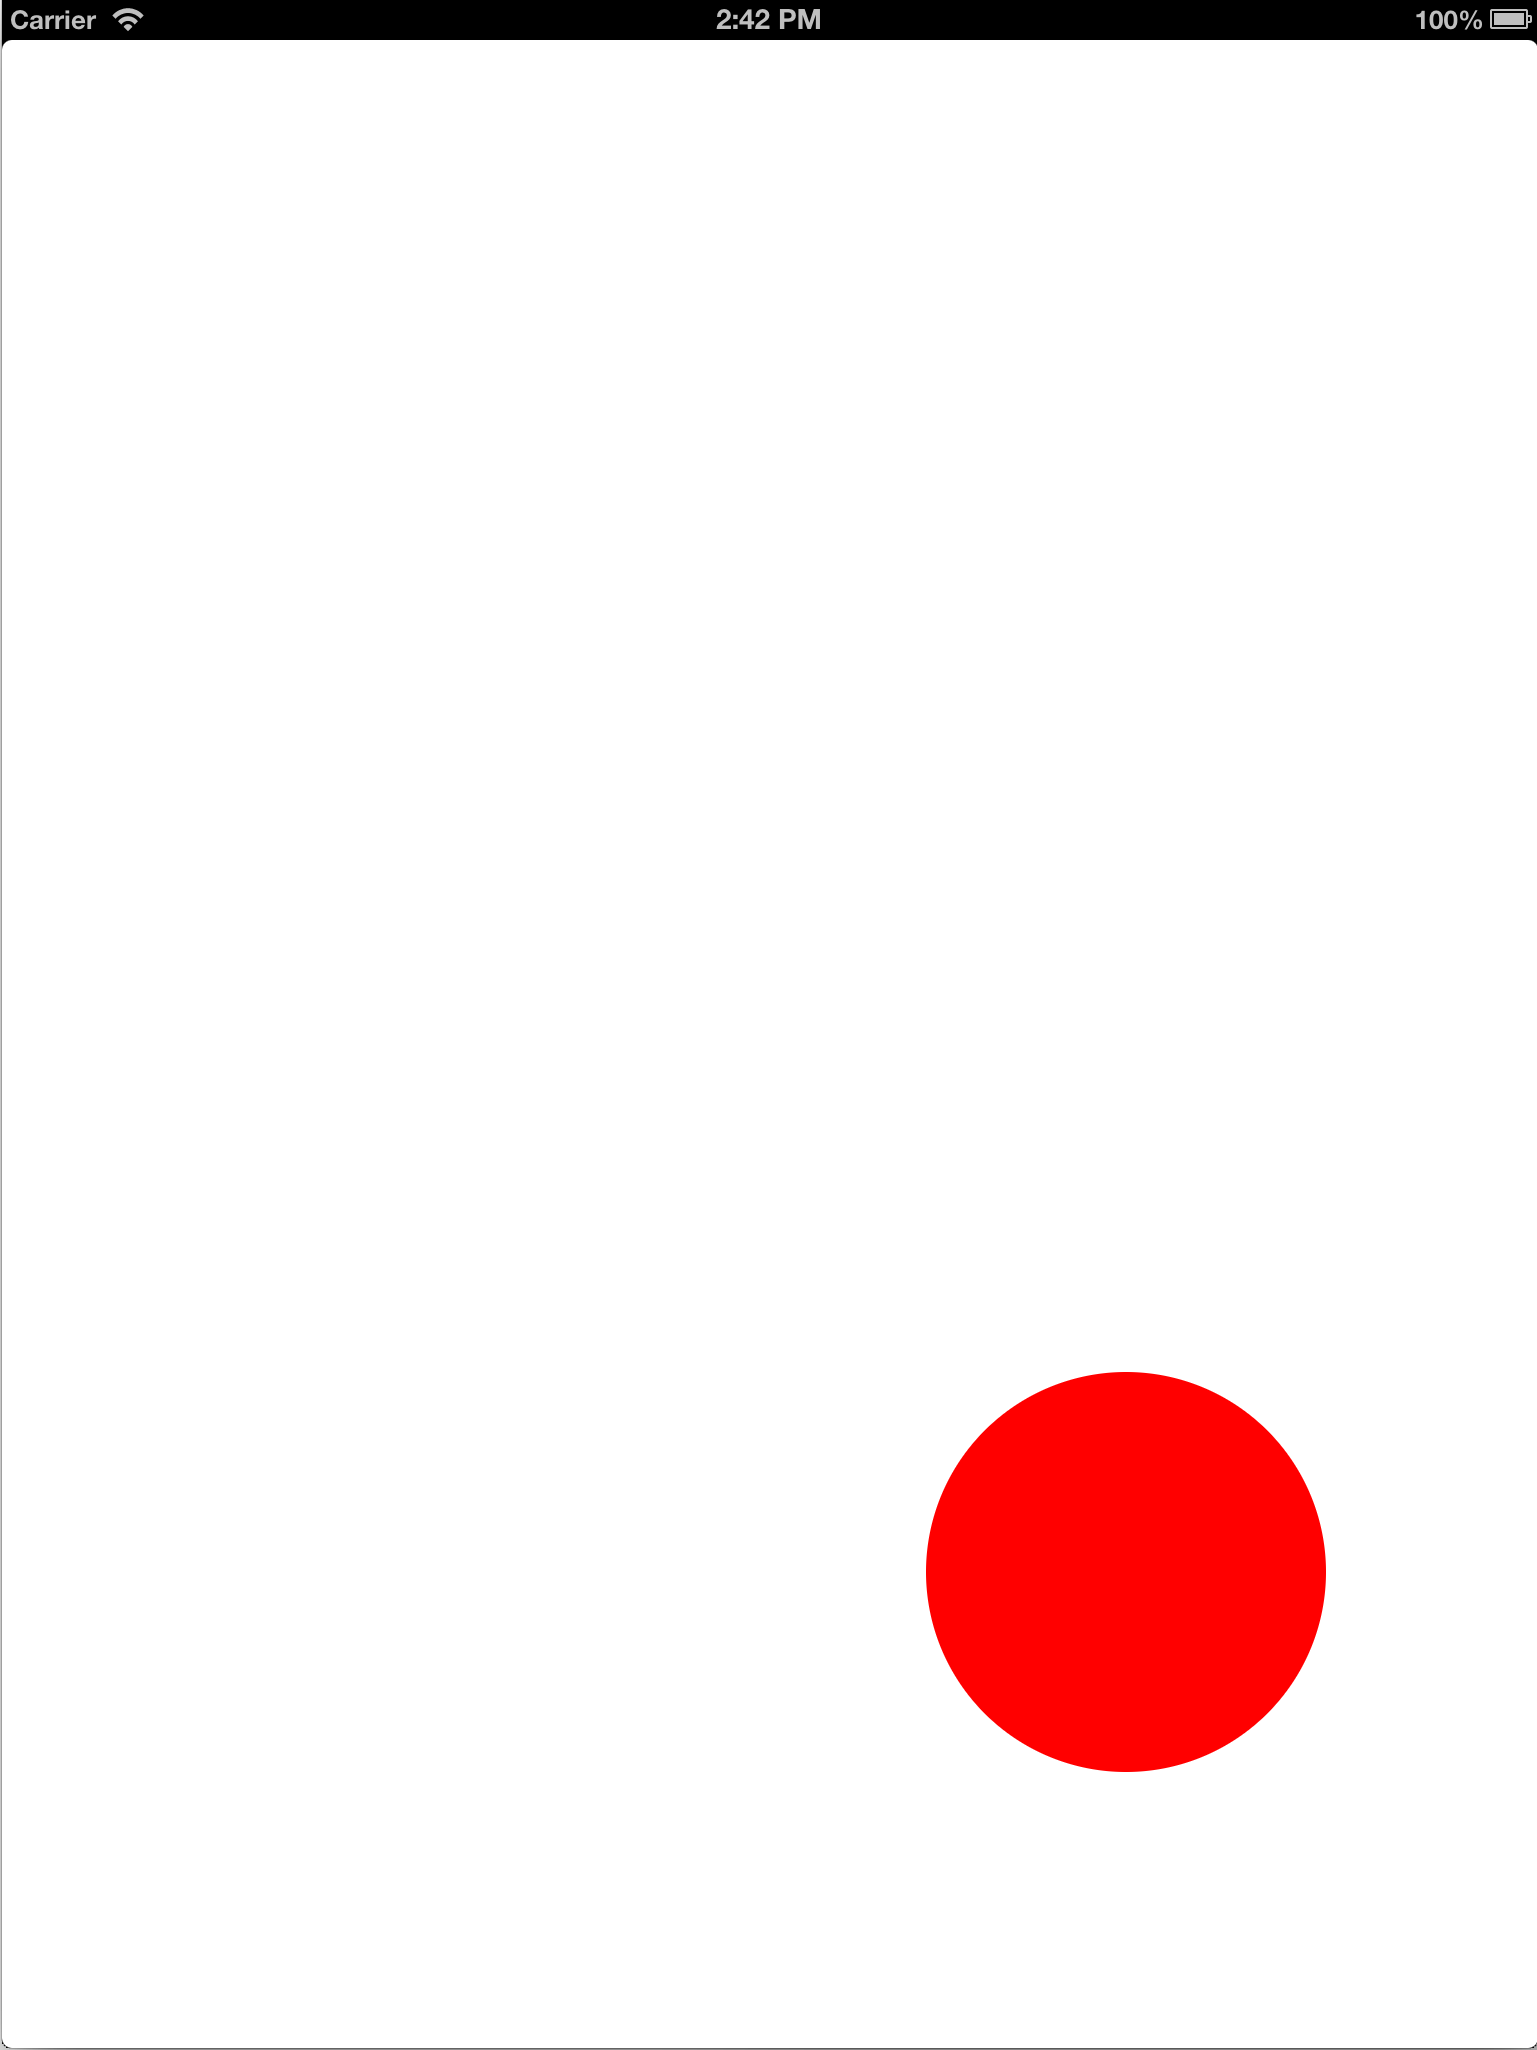
\includegraphics[width=0.45\textwidth]{test1}}}
\caption{\testfirst: in-game screenshot}
\end{figure}

\subsection{Balloon inflater}
\label{sec:test2}
The second test consisted of an application where the user was asked to inflate a balloon on the screen by tapping on it.
The balloon enlarged at every tap and shrank if not touched.
The resulting interaction is the user tapping repeatedly on the balloon in order to make it bigger, with the final result of making it explode as its dimension went beyond the screen bounds.

\begin{figure}[h!t]
\label{fig:experiment}
\centering
	{\setlength{\fboxsep}{0pt}
	 \fbox{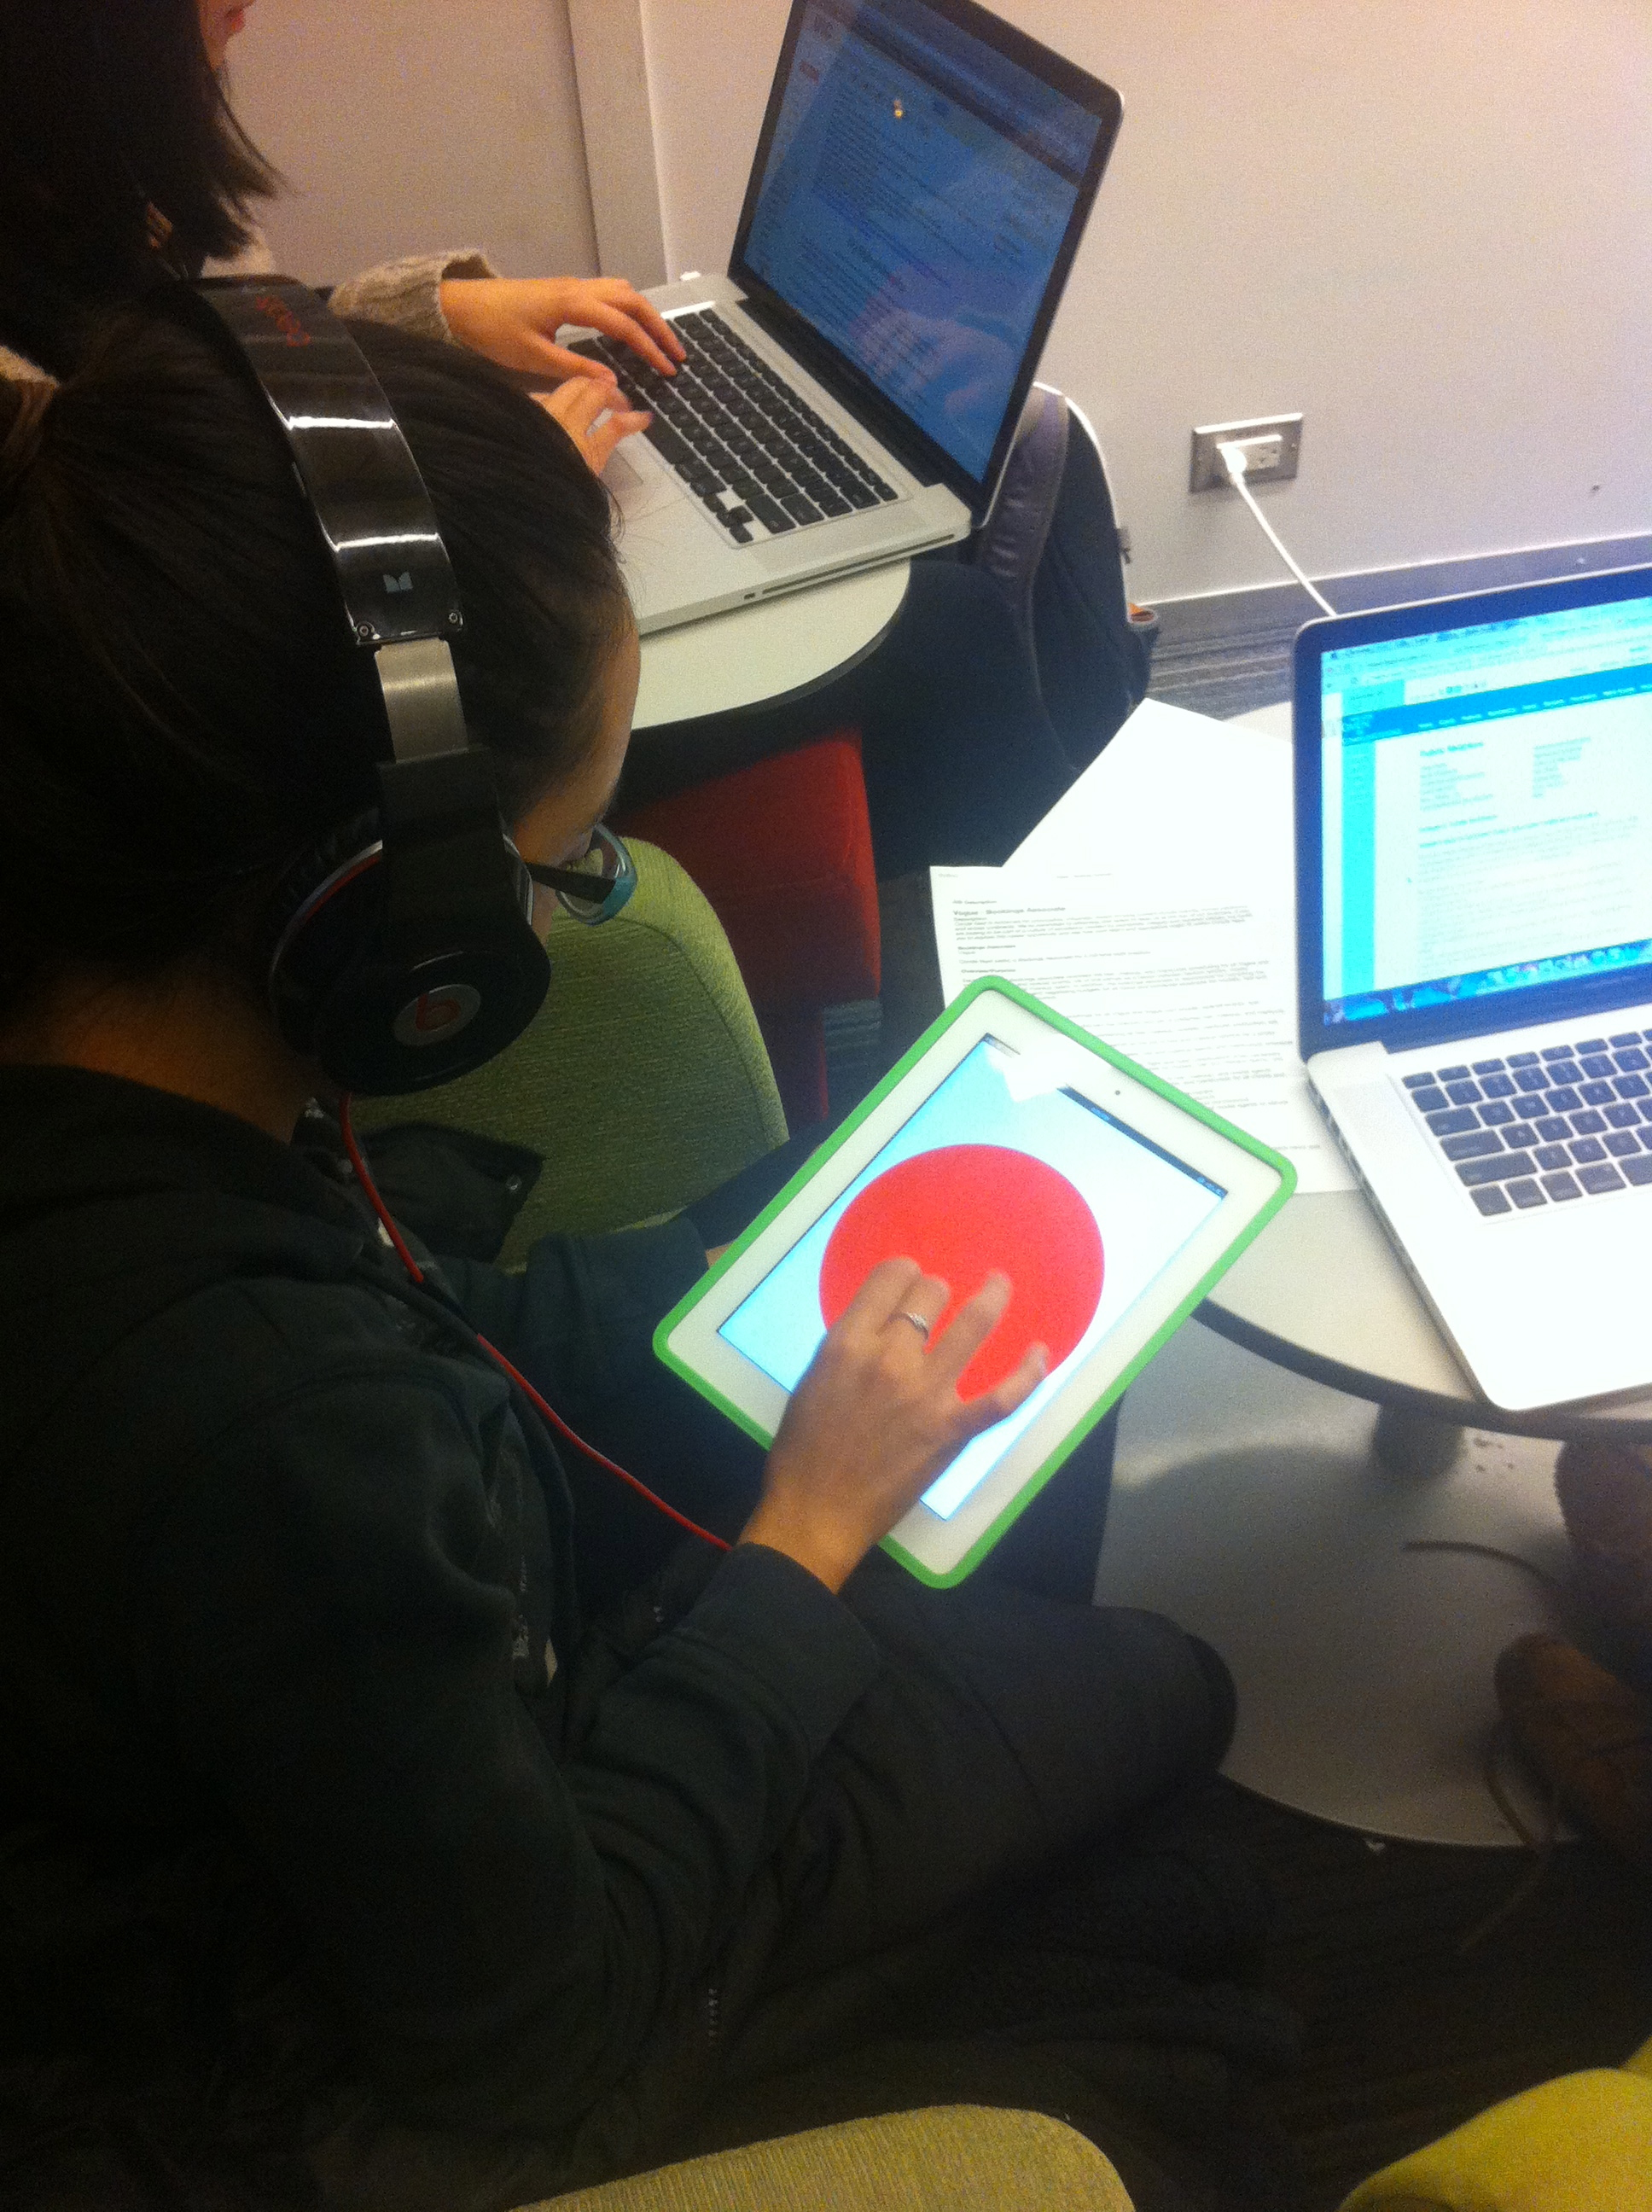
\includegraphics[width=0.45\textwidth]{experiment}}}
\caption{A tester in action}
\end{figure}

With respect to the previous test the interaction required much less cognitive activity, in the sense that the user concentration on the screen was not required in order to achieve the final result of exploding the balloon.

We will discusses later in Section~\ref{sec:conclusions} how this difference impacted on the test results.

\subsection{Data Collection}
Before moving on to the results we now present briefly how the data collection happened.

The iPad application was configured to send the data about the interaction of the user with the touchscreen to a web server we created specifically for this experiment. All the architecture has been implemented in JavaScript, taking advantage of the features of the framework Node.js.

In order to ensure that the collection was proceeding flawlessly, i.e. the data were being correctly sent to the web server, we decided to send and display them in real-time on a custom web page; the raw data were contextually stored on a MongoDB database.

The collection of raw data allowed us to avoid information loss and enabled us to perform further analysis on them.